% % % =========================================================
% % % overall_system_flow
% % % =========================================================

% \begingroup
% \hyphenpenalty=10000
% \exhyphenpenalty=10000
% \begin{tikzpicture}[x=1cm,y=1cm,>=stealth]
% \path[use as bounding box] (0,0.45) rectangle (16.00,22.55);

% % Subsystem colours, consistent with the component diagram.
% \definecolor{archline}{HTML}{26384C}
% \definecolor{aiborder}{HTML}{1261A8}
% \definecolor{aifill}{HTML}{DCEBFE}
% \definecolor{verborder}{HTML}{6842B5}
% \definecolor{verfill}{HTML}{E9DDFB}
% \definecolor{knowborder}{HTML}{338A49}
% \definecolor{knowfill}{HTML}{DDF3DF}
% \definecolor{execborder}{HTML}{B97800}
% \definecolor{execfill}{HTML}{FCE8B8}
% \definecolor{extborder}{HTML}{5B6677}
% \definecolor{extfill}{HTML}{E4E6EA}

% \tikzset{
%   flowbox/.style={rectangle,rounded corners=3pt,line width=0.7pt,
%     align=center,text=archline,font=\sffamily\fontsize{9.3}{11.2}\selectfont,
%     text width=4.30cm,minimum width=4.80cm,minimum height=1.05cm,
%     inner xsep=3pt,inner ysep=3pt,outer sep=0pt},
%   ai/.style={flowbox,draw=aiborder,fill=aifill},
%   verification/.style={flowbox,draw=verborder,fill=verfill},
%   execution/.style={flowbox,draw=execborder,fill=execfill},
%   external/.style={flowbox,draw=extborder,fill=extfill},
%   knowledge/.style={flowbox,draw=knowborder,fill=knowfill,
%     text width=3.95cm,minimum width=4.35cm,minimum height=1.45cm},
%   outcome/.style={external,text width=3.35cm,minimum width=3.75cm,
%     minimum height=1.15cm,font=\sffamily\fontsize{9}{10.8}\selectfont},
%   flowarrow/.style={->,draw=archline,line width=0.70pt},
%   arrowlabel/.style={font=\sffamily\fontsize{7.8}{9.2}\selectfont,
%     text=archline,fill=none,inner sep=0.8pt,outer sep=0pt},
%   annotation/.style={align=center,text=archline,
%     font=\sffamily\fontsize{8.4}{10}\selectfont}
% }

% % Diamond dimensions and predictable connection points.
% % Arguments: name, y, border colour, fill colour, text.
% \def\FlowDecision#1#2#3#4#5{%
%   \draw[draw=#3,fill=#4,line width=0.7pt]
%     (7.85,{#2+0.80}) -- (10.25,#2) --
%     (7.85,{#2-0.80}) -- (5.45,#2) -- cycle;
%   \node[align=center,text=archline,text width=3.40cm,
%     font=\sffamily\fontsize{9.0}{10.8}\selectfont,inner sep=0pt]
%     at (7.85,#2) {#5};
%   \coordinate (#1-north) at (7.85,{#2+0.80});
%   \coordinate (#1-south) at (7.85,{#2-0.80});
%   \coordinate (#1-east) at (10.25,#2);
% }

% % =========================================================
% % Main request-processing path
% % =========================================================
% \node[external] (request) at (7.85,21.85)
%   {Natural-Language\\DeFi Request};
% \node[ai] (generation) at (7.85,20.25)
%   {LLM-Based\\Intent Generation};
% \node[ai] (validation) at (7.85,18.65)
%   {Intent Validation};
% \FlowDecision{intent}{16.95}{aiborder}{aifill}
%   {Intent valid?}

% \draw[flowarrow] (request.south) -- (generation.north);
% \draw[flowarrow] (generation.south) --
%   node[arrowlabel,pos=0.5,right=3pt] {Candidate intent}
%   (validation.north);
% \draw[flowarrow] (validation.south) -- (intent-north);

% \node[outcome] (intentfailure) at (13.50,16.95)
%   {Clarify or Reject\\Execution Blocked};
% \draw[flowarrow] (intent-east) --
%   node[arrowlabel,pos=0.5,above=3pt] {No} (intentfailure.west);

% \node[verification] (verify) at (7.85,14.90)
%   {Action-Specific\\Relationship Verification};
% \draw[flowarrow] (intent-south) --
%   node[arrowlabel,pos=0.5,right=3pt] {Yes} (verify.north);

% \FlowDecision{evidence}{12.85}{verborder}{verfill}
%   {Evidence sufficient\\and current?}
% \draw[flowarrow] (verify.south) -- (evidence-north);
% \node[outcome] (insufficient) at (13.50,12.85)
%   {Verification Failure\\Execution Blocked};
% \draw[flowarrow] (evidence-east) --
%   node[arrowlabel,pos=0.5,above=3pt] {No} (insufficient.west);

% \FlowDecision{relationships}{10.50}{verborder}{verfill}
%   {Required relationships\\established?}
% \draw[flowarrow] (evidence-south) --
%   node[arrowlabel,pos=0.5,right=3pt] {Yes} (relationships-north);
% \node[outcome] (rejection) at (13.50,10.50)
%   {\textbf{REJECT}\\Execution Blocked};
% \draw[flowarrow] (relationships-east) --
%   node[arrowlabel,pos=0.5,above=3pt] {No} (rejection.west);

% \node[verification] (approved) at (7.85,8.45)
%   {\textbf{APPROVE}\\Structured Verification Result};
% \draw[flowarrow] (relationships-south) --
%   node[arrowlabel,pos=0.5,right=3pt] {Yes} (approved.north);

% % Includes the pre-execution check of the approved result.
% \FlowDecision{valid}{6.40}{execborder}{execfill}
%   {Verified result\\still valid?}
% \draw[flowarrow] (approved.south) -- (valid-north);
% \node[outcome] (reverify) at (13.50,6.40)
%   {Reverification Required\\Execution Blocked};
% \draw[flowarrow] (valid-east) --
%   node[arrowlabel,pos=0.5,above=3pt] {No} (reverify.west);

% \node[execution] (execution) at (7.85,4.325)
%   {Controlled Smart-Wallet\\Execution (ERC-4337)};
% \draw[flowarrow] (valid-south) --
%   node[arrowlabel,pos=0.5,right=3pt] {Yes} (execution.north);
% \node[outcome] (submissionfailure) at (13.50,4.325)
%   {Submission Rejected\\or Failed};
% \draw[flowarrow] (execution.east) --
%   node[arrowlabel,pos=0.5,above=3pt] {Failure} (submissionfailure.west);

% \node[external] (chain) at (7.85,2.675)
%   {Blockchain Network};
% \draw[flowarrow] (execution.south) --
%   node[arrowlabel,pos=0.5,right=3pt] {Transaction} (chain.north);

% % =========================================================
% % Independent knowledge branch
% % =========================================================
% \node[external,text width=3.95cm,minimum width=4.35cm]
%   (sources) at (2.50,20.25) {Authoritative DeFi\\Sources};
% \node[knowledge] (acquisition) at (2.50,18.30)
%   {Knowledge Acquisition,\\Admission and\\Maintenance};
% \node[knowledge] (graph) at (2.50,16.25)
%   {Authoritative Verification\\Knowledge\\(Property Graph)};
% \draw[flowarrow] (sources.south) -- (acquisition.north);
% \draw[flowarrow] (acquisition.south) --
%   node[arrowlabel,pos=0.5,left=3pt] {Accepted updates} (graph.north);
% \draw[flowarrow] (graph.east) -- (5.075,16.25) --
%   (5.075,14.90) -- (verify.west);
% \node[annotation,text width=4.20cm] at (2.50,14.45)
%   {Maintained independently};

% % =========================================================
% % One-row legend: aligned swatches and labels
% % =========================================================
% \begingroup

% \def\LegendSwatch#1#2{%
%   \tikz[baseline=-0.5ex]{%
%     \draw[
%       draw=#1,
%       fill=#2,
%       rounded corners=1pt,
%       line width=0.5pt
%     ] (0,0) rectangle (0.26,0.26);
%   }%
%   \hspace{4pt}%
% }

% \draw[draw=extborder,rounded corners=3pt,line width=0.6pt]
%   (0.35,0.65) rectangle (15.50,1.50);

% \node[
%   font=\sffamily\fontsize{8.5}{10}\selectfont,
%   text=archline,
%   inner sep=0pt,
%   outer sep=0pt
% ] at (7.925,1.075) {%
%   \resizebox{14.55cm}{!}{%
%     \begin{tabular}{
%       @{}l@{\hspace{12pt}}
%       l@{\hspace{12pt}}
%       l@{\hspace{12pt}}
%       l@{\hspace{12pt}}
%       l@{}
%     }
%       \LegendSwatch{aiborder}{aifill} AI / Intent Processing
%       &
%       \LegendSwatch{verborder}{verfill} Relationship Verification
%       &
%       \LegendSwatch{knowborder}{knowfill} Verification Knowledge
%       &
%       \LegendSwatch{execborder}{execfill} Controlled Execution
%       &
%       \LegendSwatch{extborder}{extfill} External / Outcomes
%     \end{tabular}%
%   }%
% };

% \endgroup
% \end{tikzpicture}
% \endgroup

% Conceptual request flow with UML-style initial and final nodes.
% Independent knowledge maintenance is supporting context, outside the request activity.
% Preamble: \usepackage{tikz} and \usepackage{graphicx}
% Include this file with \input{figures/overall_system_flow_with_notation.tex}.
\begingroup
\hyphenpenalty=10000
\exhyphenpenalty=10000
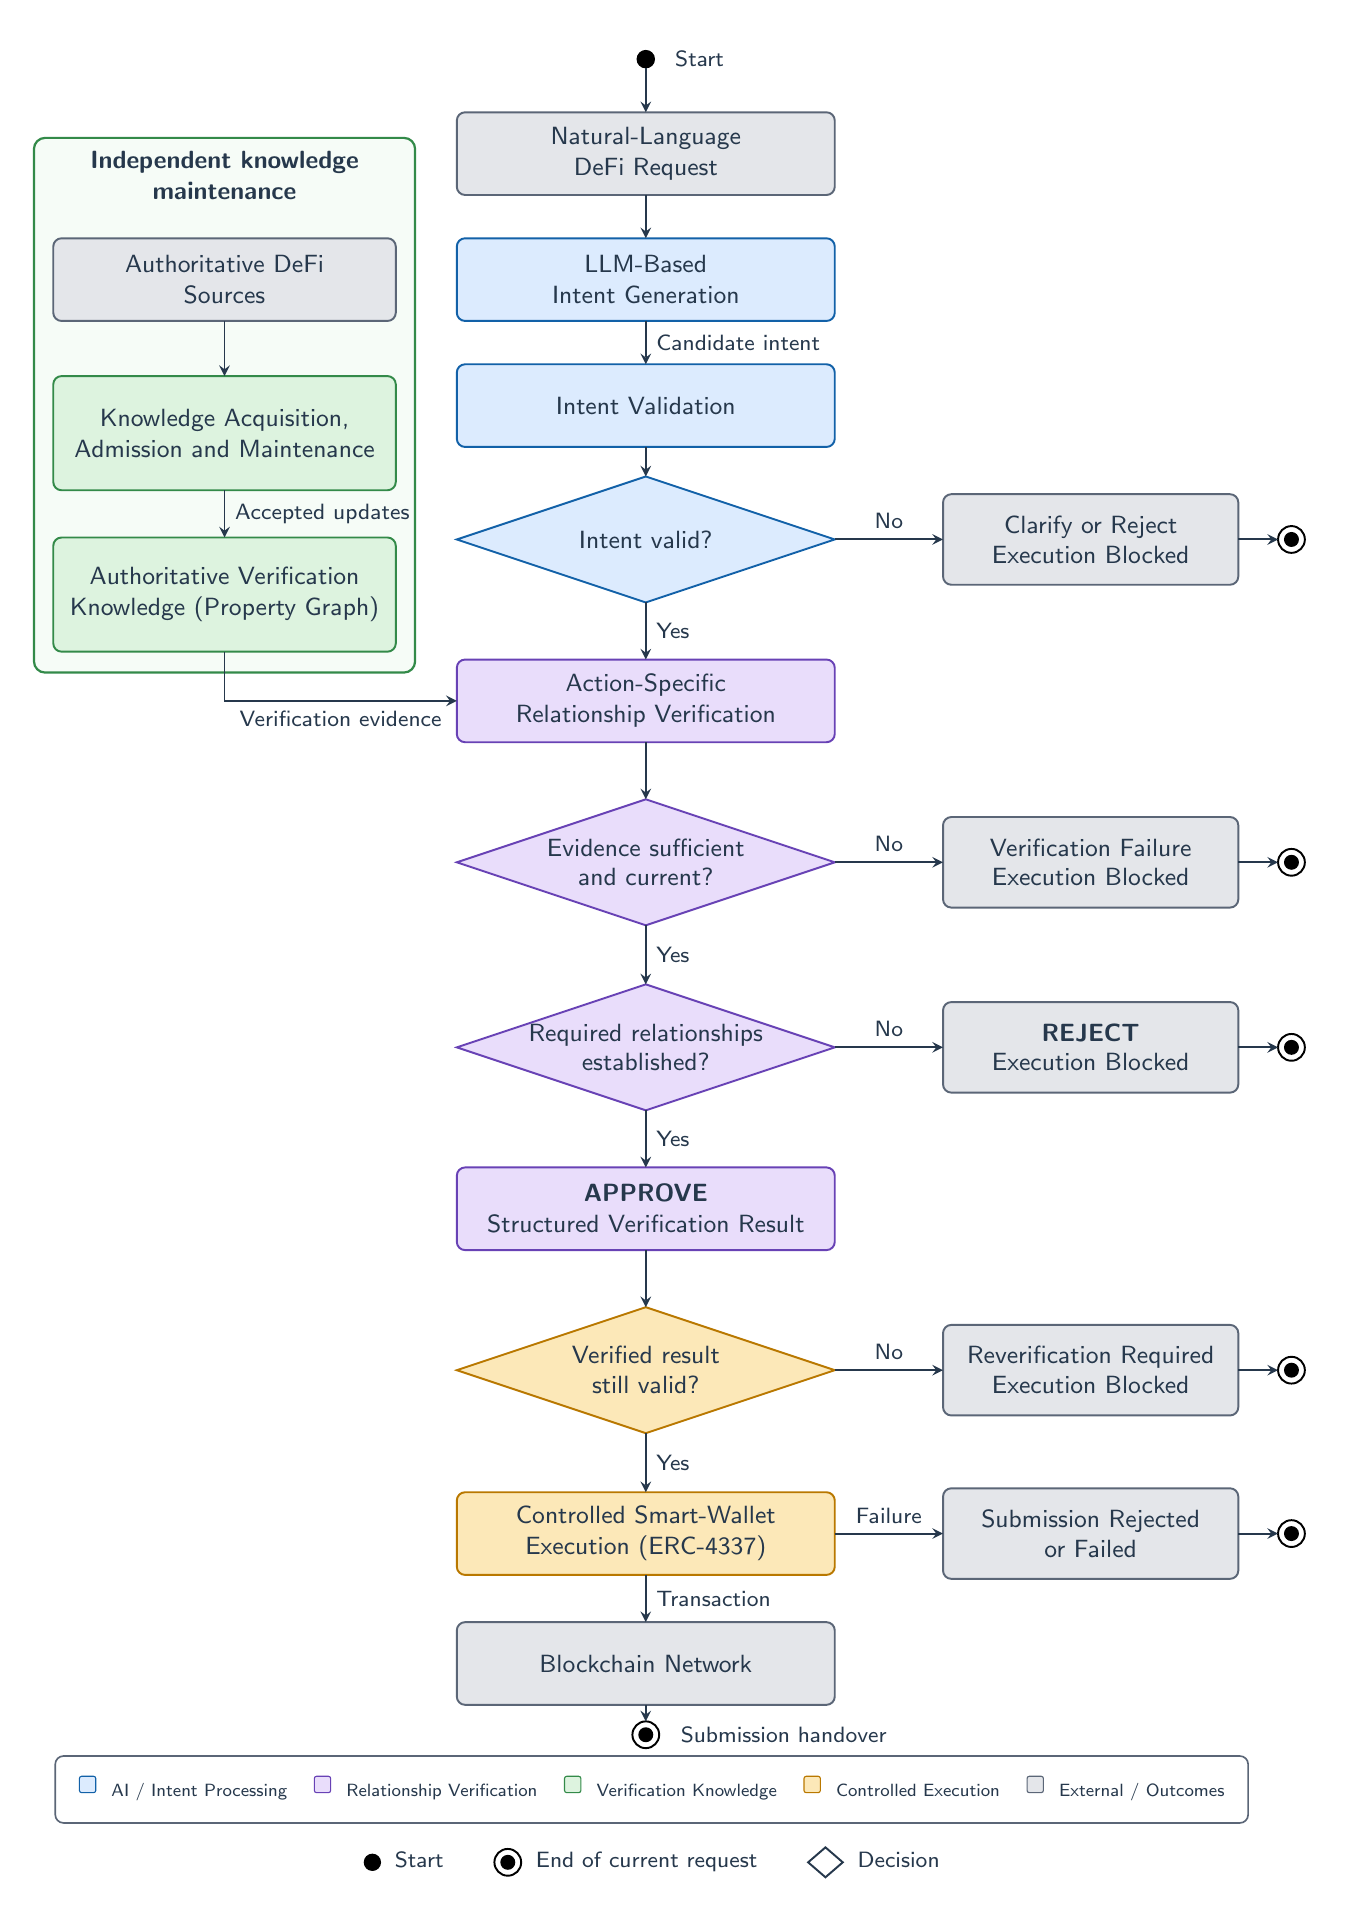
\begin{tikzpicture}[x=1cm,y=1cm,>=stealth]
\path[use as bounding box] (0,-0.20) rectangle (16.55,23.45);

% Subsystem colours, consistent with the component diagram.
\definecolor{archline}{HTML}{26384C}
\definecolor{aiborder}{HTML}{1261A8}
\definecolor{aifill}{HTML}{DCEBFE}
\definecolor{verborder}{HTML}{6842B5}
\definecolor{verfill}{HTML}{E9DDFB}
\definecolor{knowborder}{HTML}{338A49}
\definecolor{knowfill}{HTML}{DDF3DF}
\definecolor{execborder}{HTML}{B97800}
\definecolor{execfill}{HTML}{FCE8B8}
\definecolor{extborder}{HTML}{5B6677}
\definecolor{extfill}{HTML}{E4E6EA}

\tikzset{
  flowbox/.style={rectangle,rounded corners=3pt,line width=0.7pt,
    align=center,text=archline,font=\sffamily\fontsize{9.3}{11.2}\selectfont,
    text width=4.30cm,minimum width=4.80cm,minimum height=1.05cm,
    inner xsep=3pt,inner ysep=3pt,outer sep=0pt},
  ai/.style={flowbox,draw=aiborder,fill=aifill},
  verification/.style={flowbox,draw=verborder,fill=verfill},
  execution/.style={flowbox,draw=execborder,fill=execfill},
  external/.style={flowbox,draw=extborder,fill=extfill},
  knowledge/.style={flowbox,draw=knowborder,fill=knowfill,
    text width=3.95cm,minimum width=4.35cm,minimum height=1.45cm},
  outcome/.style={external,text width=3.35cm,minimum width=3.75cm,
    minimum height=1.15cm,font=\sffamily\fontsize{9}{10.8}\selectfont},
  flowarrow/.style={->,draw=archline,line width=0.70pt},
  arrowlabel/.style={font=\sffamily\fontsize{7.8}{9.2}\selectfont,
    text=archline,fill=none,inner sep=0.8pt,outer sep=0pt},
  annotation/.style={align=center,text=archline,
    font=\sffamily\fontsize{8.4}{10}\selectfont}
}

% Diamond dimensions and predictable connection points.
% Arguments: name, y, border colour, fill colour, text.
\def\FlowDecision#1#2#3#4#5{%
  \draw[draw=#3,fill=#4,line width=0.7pt]
    (7.85,{#2+0.80}) -- (10.25,#2) --
    (7.85,{#2-0.80}) -- (5.45,#2) -- cycle;
  \node[align=center,text=archline,text width=3.40cm,
    font=\sffamily\fontsize{9.0}{10.8}\selectfont,inner sep=0pt]
    at (7.85,#2) {#5};
  \coordinate (#1-north) at (7.85,{#2+0.80});
  \coordinate (#1-south) at (7.85,{#2-0.80});
  \coordinate (#1-east) at (10.25,#2);
}

% =========================================================
% Main request-processing path
% =========================================================
% UML-style initial node for one request-processing attempt.
\node[circle,draw=black,fill=black,minimum size=0.22cm,
  inner sep=0pt,outer sep=0pt] (requeststart) at (7.85,23.05) {};
\node[annotation,anchor=west] at (8.10,23.05) {Start};

\node[external] (request) at (7.85,21.85)
  {Natural-Language\\DeFi Request};
\node[ai] (generation) at (7.85,20.25)
  {LLM-Based\\Intent Generation};
\node[ai] (validation) at (7.85,18.65)
  {Intent Validation};
\FlowDecision{intent}{16.95}{aiborder}{aifill}
  {Intent valid?}

\draw[flowarrow] (requeststart.south) -- (request.north);
\draw[flowarrow] (request.south) -- (generation.north);
\draw[flowarrow] (generation.south) --
  node[arrowlabel,pos=0.5,right=3pt] {Candidate intent}
  (validation.north);
\draw[flowarrow] (validation.south) -- (intent-north);

\node[outcome] (intentfailure) at (13.50,16.95)
  {Clarify or Reject\\Execution Blocked};
\draw[flowarrow] (intent-east) --
  node[arrowlabel,pos=0.5,above=3pt] {No} (intentfailure.west);

\node[verification] (verify) at (7.85,14.90)
  {Action-Specific\\Relationship Verification};
\draw[flowarrow] (intent-south) --
  node[arrowlabel,pos=0.5,right=3pt] {Yes} (verify.north);

\FlowDecision{evidence}{12.85}{verborder}{verfill}
  {Evidence sufficient\\and current?}
\draw[flowarrow] (verify.south) -- (evidence-north);
\node[outcome] (insufficient) at (13.50,12.85)
  {Verification Failure\\Execution Blocked};
\draw[flowarrow] (evidence-east) --
  node[arrowlabel,pos=0.5,above=3pt] {No} (insufficient.west);

\FlowDecision{relationships}{10.50}{verborder}{verfill}
  {Required relationships\\established?}
\draw[flowarrow] (evidence-south) --
  node[arrowlabel,pos=0.5,right=3pt] {Yes} (relationships-north);
\node[outcome] (rejection) at (13.50,10.50)
  {\textbf{REJECT}\\Execution Blocked};
\draw[flowarrow] (relationships-east) --
  node[arrowlabel,pos=0.5,above=3pt] {No} (rejection.west);

\node[verification] (approved) at (7.85,8.45)
  {\textbf{APPROVE}\\Structured Verification Result};
\draw[flowarrow] (relationships-south) --
  node[arrowlabel,pos=0.5,right=3pt] {Yes} (approved.north);

% Includes the pre-execution check of the approved result.
\FlowDecision{valid}{6.40}{execborder}{execfill}
  {Verified result\\still valid?}
\draw[flowarrow] (approved.south) -- (valid-north);
\node[outcome] (reverify) at (13.50,6.40)
  {Reverification Required\\Execution Blocked};
\draw[flowarrow] (valid-east) --
  node[arrowlabel,pos=0.5,above=3pt] {No} (reverify.west);

\node[execution] (execution) at (7.85,4.325)
  {Controlled Smart-Wallet\\Execution (ERC-4337)};
\draw[flowarrow] (valid-south) --
  node[arrowlabel,pos=0.5,right=3pt] {Yes} (execution.north);
\node[outcome] (submissionfailure) at (13.50,4.325)
  {Submission Rejected\\or Failed};
\draw[flowarrow] (execution.east) --
  node[arrowlabel,pos=0.5,above=3pt] {Failure} (submissionfailure.west);

\node[external] (chain) at (7.85,2.675)
  {Blockchain Network};
\draw[flowarrow] (execution.south) --
  node[arrowlabel,pos=0.5,right=3pt] {Transaction} (chain.north);

% UML-style activity-final nodes end the current request attempt.
% They do not stop the independently maintained knowledge subsystem.
\def\FlowRequestEnd#1#2#3{%
  \node[circle,draw=black,fill=white,line width=0.7pt,
    minimum size=0.34cm,inner sep=0pt,outer sep=0pt]
    (#1) at (#2,#3) {};
  \fill[black] (#1.center) circle[radius=0.095cm];
}

\FlowRequestEnd{intentend}{16.05}{16.95}
\draw[flowarrow] (intentfailure.east) -- (intentend.west);

\FlowRequestEnd{evidenceend}{16.05}{12.85}
\draw[flowarrow] (insufficient.east) -- (evidenceend.west);

\FlowRequestEnd{rejectionend}{16.05}{10.50}
\draw[flowarrow] (rejection.east) -- (rejectionend.west);

\FlowRequestEnd{reverifyend}{16.05}{6.40}
\draw[flowarrow] (reverify.east) -- (reverifyend.west);

\FlowRequestEnd{submissionend}{16.05}{4.325}
\draw[flowarrow] (submissionfailure.east) -- (submissionend.west);

% This endpoint denotes handover for submission, not confirmed execution.
\FlowRequestEnd{handoverend}{7.85}{1.77}
\draw[flowarrow] (chain.south) -- (handoverend.north);
\node[annotation,anchor=west] at (8.17,1.77) {Submission handover};

% % =========================================================
% % Independent knowledge branch
% % =========================================================
% \node[external,text width=3.95cm,minimum width=4.35cm]
%   (sources) at (2.50,20.25) {Authoritative DeFi\\Sources};
% \node[knowledge] (acquisition) at (2.50,18.30)
%   {Knowledge Acquisition,\\Admission and\\Maintenance};
% \node[knowledge] (graph) at (2.50,16.25)
%   {Authoritative Verification\\Knowledge\\(Property Graph)};
% \draw[flowarrow] (sources.south) -- (acquisition.north);
% \draw[flowarrow] (acquisition.south) --
%   node[arrowlabel,pos=0.5,left=3pt] {Accepted updates} (graph.north);
% \draw[flowarrow] (graph.east) -- (5.075,16.25) --
%   (5.075,14.90) -- (verify.west);
% \node[annotation,text width=4.20cm] at (2.50,14.45)
%   {Maintained independently};

% =========================================================
% Independent knowledge maintenance
% =========================================================

% Separate panel: this process runs independently of user requests.
\draw[
  draw=knowborder,
  fill=knowfill!25!white,
  rounded corners=4pt,
  line width=0.8pt
] (0.08,15.26) rectangle (4.92,22.05);

\node[
  align=center,
  text=archline,
  font=\sffamily\bfseries\fontsize{9.3}{11.2}\selectfont,
  inner sep=0pt
] at (2.50,21.58) {Independent knowledge \\ maintenance};

% Existing knowledge stages, in their original colours.
\node[external,text width=3.95cm,minimum width=4.35cm]
  (sources) at (2.50,20.25)
  {Authoritative DeFi\\Sources};

\node[knowledge]
  (acquisition) at (2.50,18.30)
  {Knowledge Acquisition,\\Admission and Maintenance};

\node[knowledge]
  (graph) at (2.50,16.25)
  {Authoritative Verification\\Knowledge (Property Graph)};

\draw[flowarrow]
  (sources.south) -- (acquisition.north);

\draw[flowarrow]
  (acquisition.south) --
  node[arrowlabel,midway,right=3pt] {Accepted updates}
  (graph.north);

% The verifier uses evidence from the maintained graph.
% Route below the panel so the label stays clear of its border.
\draw[flowarrow]
  (graph.south) -- (2.50,14.90) --
  node[arrowlabel,midway,below=3pt] {Verification evidence}
  (verify.west);

% =========================================================
% One-row legend: aligned swatches and labels
% =========================================================
\begingroup

\def\LegendSwatch#1#2{%
  \tikz[baseline=-0.5ex]{%
    \draw[
      draw=#1,
      fill=#2,
      rounded corners=1pt,
      line width=0.5pt
    ] (0,0) rectangle (0.26,0.26);
  }%
  \hspace{4pt}%
}

\draw[draw=extborder,rounded corners=3pt,line width=0.6pt]
  (0.35,0.65) rectangle (15.50,1.50);

\node[
  font=\sffamily\fontsize{8.5}{10}\selectfont,
  text=archline,
  inner sep=0pt,
  outer sep=0pt
] at (7.925,1.075) {%
  \resizebox{14.55cm}{!}{%
    \begin{tabular}{
      @{}l@{\hspace{12pt}}
      l@{\hspace{12pt}}
      l@{\hspace{12pt}}
      l@{\hspace{12pt}}
      l@{}
    }
      \LegendSwatch{aiborder}{aifill} AI / Intent Processing
      &
      \LegendSwatch{verborder}{verfill} Relationship Verification
      &
      \LegendSwatch{knowborder}{knowfill} Verification Knowledge
      &
      \LegendSwatch{execborder}{execfill} Controlled Execution
      &
      \LegendSwatch{extborder}{extfill} External / Outcomes
    \end{tabular}%
  }%
};

\endgroup

% Compact, centred UML-style notation key
\node[
  annotation,
  inner sep=0pt,
  outer sep=0pt
] at (7.925,0.15) {%
  \begin{tabular}{
    @{}c@{\hspace{5pt}}l
    @{\hspace{18pt}}
    c@{\hspace{5pt}}l
    @{\hspace{18pt}}
    c@{\hspace{5pt}}l@{}
  }
    % Start
    \tikz[baseline=-0.5ex]{
      \fill[black] (0,0) circle[radius=0.11cm];
    }
    & Start
    &
    % End
    \tikz[baseline=-0.5ex]{
      \draw[draw=black,fill=white,line width=0.7pt]
        (0,0) circle[radius=0.17cm];
      \fill[black] (0,0) circle[radius=0.095cm];
    }
    & End of current request
    &
    % Decision
    \tikz[baseline=-0.5ex]{
      \draw[draw=archline,fill=white,line width=0.7pt]
        (0,0.19) -- (0.22,0) -- (0,-0.19) --
        (-0.22,0) -- cycle;
    }
    & Decision
  \end{tabular}%
};

\end{tikzpicture}
\endgroup